\chapter{State of the Art}\label{chap:state-of-the-art}
This chapter presents the current stage of the technologies related to our application, specifically the different kinds of simulators that are currently present in the market (\sectionref{sec:assembly-simulators}), both specific to one architecture (\subsectionref{subsec:specific-assembly-simulators}) and architecture-agnostic simulators (\subsectionref{subsec:generic-assembly-simulators}).\\
Finally, it includes a comparison between all the mentioned simulators and our proposed application (\sectionref{sec:comparison}).



\section{Assembly simulators}\label{sec:assembly-simulators}
An `\gls{assembly simulator}' is a CPU simulator that enables the user to program it through an \gls{assembly}, and it usually has an educational purpose: either to aid the user in learning the language, or as an exercise for the programmer in order to give them a better understanding of CPU architecture and software development.

These simulators typically offer an interface that allows the user to execute the program step-by-step and see the current state of the simulated \gls{computer}.


\subsection{Specific simulators}\label{subsec:specific-assembly-simulators}
The vast majority of simulators that can be found today focus on emulating a specific CPU architecture and set of instructions, which can range from simple 8-bit microprocessors like the Intel 8080\supercite{i8080emulator} to architectures that are used today, like \gls{ARM}\supercite{QtARMSim}.

\noindent
Here, we'll focus on two examples: Kite\supercite{song_kite2019} and ARMLite\supercite{ARMLite}.


\subsubsection*{Kite}  % Kite: https://github.com/yonseicasl/Kite
Kite\supercite{song_kite2019} is a simulator that models a five-stage \gls{pipeline} \gls{RISC-V} CPU, based on the model described in \textit{Computer organization and design: the hardware/software interface (RISC-V edition)}\supercite{PattersonDavidA.2018Coad}, by D. Patterson and J. Hennessy, and implemented in C/C++. It was developed in 2019 in order to provide students of Yonsei University (Seoul, Korea) with an easy-to use simulator to accompany follow its Computer Architecture course.

It incorporates advanced features derived from a \gls{pipeline} architecture, such as \gls{instruction dependency} detection and \gls{pipeline stalls}, among others. These `under the hood' features offer a better understanding of the underlying concepts of computer architecture.

The simulator consists of an executable with a \gls{CLI} that takes three input files: the program's code, the register's state, and the data memory's state. It loads the state of registers and data memory, executes the program's code and saves the state to the specified files, after the execution, printing some statistics (Figure \ref{fig:kite}). It also implements a \gls{debug} mode that prints the state of each instruction on the \gls{pipeline}, each \gls{clock cycle}.

\begin{figure}[h]
  \caption{Kite simulator \gls{CLI}.}
  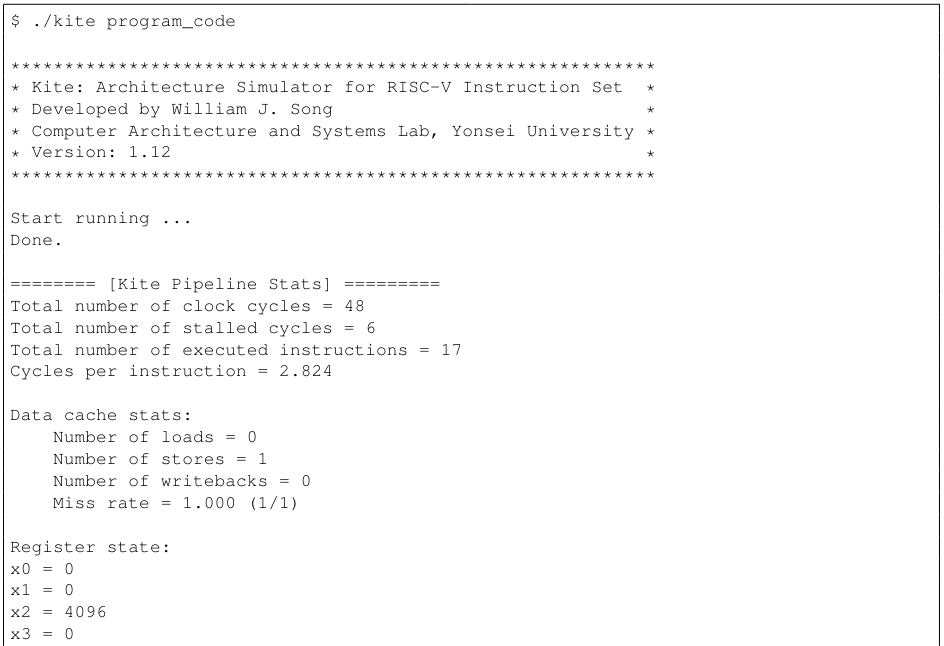
\includegraphics[width=0.7\textwidth]{kite.png}
  \label{fig:kite}
\end{figure}


% \subsubsection*{MARS}  % https://courses.missouristate.edu/KenVollmar/MARS/index.htm
% MARS\supercite{VollmarKenneth2006MaeM} follows the \gls{MIPS} architecture, another \gls{RISC} type architecture.

\subsection*{ARMLite}  % https://www.peterhigginson.co.uk/ARMlite/
ARMLite\supercite{ARMLite} is a web-based simulator for a 32-bit `\glsdisp{ARM}{ARM-like}' processor. It includes a basic set of instructions described in \textit{Assembly Language Programming}\supercite{PawsonRichard.2020Ass}, by R. Pawson.


\subsection{Generic simulators}\label{subsec:generic-assembly-simulators}


% CREATOR: https://creatorsim.github.io/

% sail




\section{Comparison}\label{sec:comparison}


\begin{table}[h]
  \caption{Feature comparison of current assembly simulators.}
  \tiny  % too big to use normal font
  \resizebox{\textwidth}{!}{  % fit to textwidth
    % \begin{tabular}{>{\bfseries}p{3cm}|M{1.7cm}M{1.7cm}M{1.7cm}M{1.7cm}M{1.7cm}M{1.7cm}}
    % \begin{tabular}{>{\bfseries}m{3cm}cccccc}
    \begin{tabular}{>{\bfseries}lccccc}
      \hline
      Simulator   & Kite       & ARMLite    & CREATOR    & Sail       & Proposal\\
      \hline
      Language    & C/C++      & JavaScript & JavaScript & OCaml      & C++23\\
      \gls{FOSS}  & \checkmark & \checkmark\tablefootnote{While we couldn't find any information about the license used by this simulator, the webpage it runs in has its source code \glsdisp{obfuscate}{unobfuscated} and is, to date, public and free to use.}
                                            & \checkmark & \checkmark & \checkmark\\
      Architecture definition file 
                  &            &            & \checkmark & \checkmark\tablefootnote{Simulator needs to be \glsdisp{compilation}{recompiled} for any new architecture.} 
                                                                      & \checkmark\\
      Execute files
                  & \checkmark &            & \checkmark &            & \checkmark\\
      \gls{CLI}   & \checkmark &            & \checkmark & \checkmark & \checkmark\\
      Step-by-step execution
                  &            &            & \checkmark & \checkmark & \checkmark\\
      Simple \& generic language 
                  &            &            &            &            & \checkmark\\
      \hline
    \end{tabular}
  }
\end{table}